\chapter{Indústria brasileira de Jogos Eletrônicos}

A indústria de jogos no Brasil tem se consolidado como um dos maiores mercados consumidores do mundo, ocupando atualmente a quinta posição global em consumo de jogos eletrônicos. Dados recentes apontam que 89,8\% da população brasileira consome jogos regularmente (\cite{internetGame:share}), utilizando dispositivos móveis, consoles e computadores como principais plataformas. Essa alta adesão reflete a popularidade dos jogos eletrônicos no país, que ultrapassaram a barreira do entretenimento e se tornaram parte do cotidiano de grande parte dos brasileiros.

Entretanto, apesar da expressiva participação no consumo, o Brasil enfrenta desafios significativos quando se trata de publicação de jogos. Publicadoras de jogos, responsáveis por financiar, distribuir e promover os títulos no mercado, desempenham um papel crucial no sucesso de um jogo. Essas empresas frequentemente definem o alcance e o impacto que um título pode ter globalmente. Contudo, o Brasil não figura nem entre os dez principais países que mais publicam jogos (\cite{publishers:country}), evidenciando uma lacuna significativa entre o consumo e a produção nacional.

\begin{figure}[H]
    \centering
    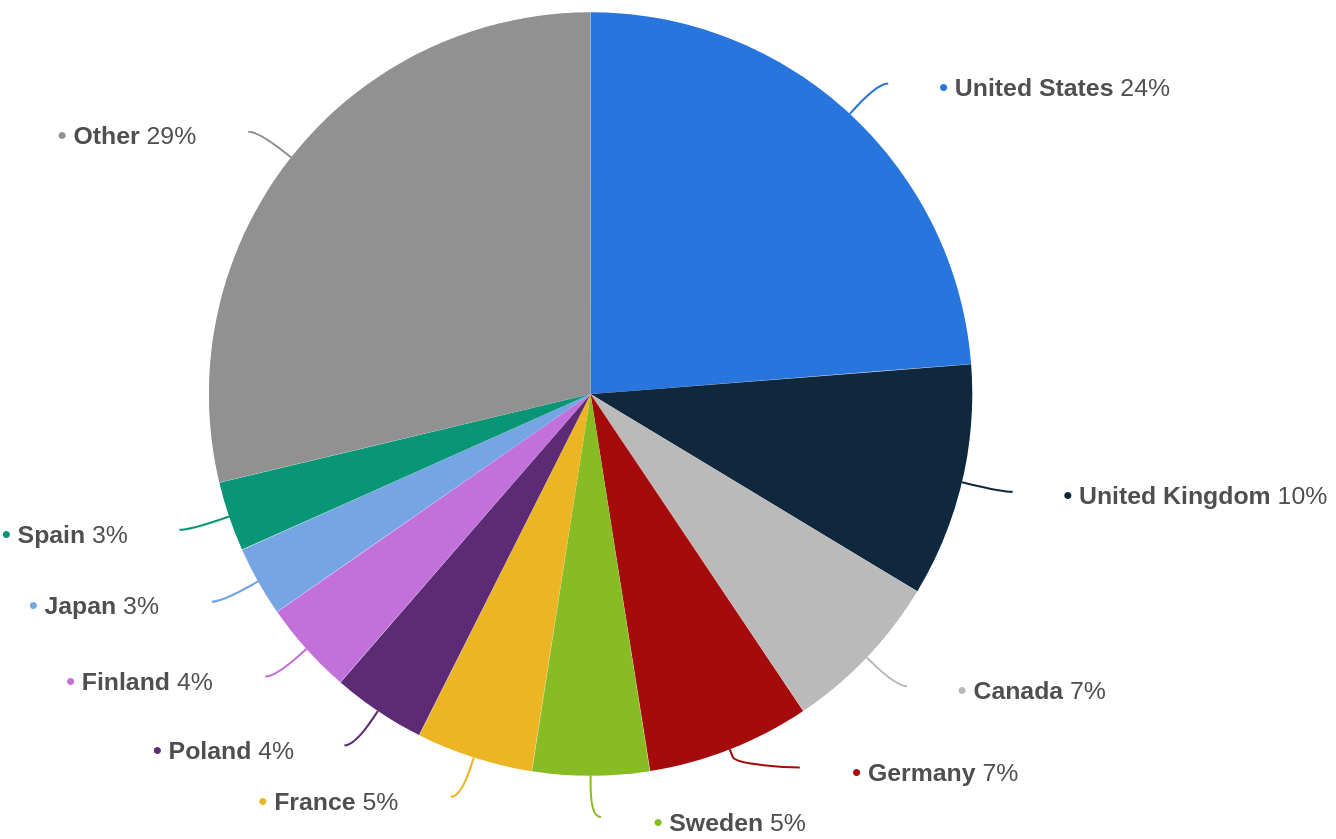
\includegraphics[width=0.8\textwidth]{figuras/Devs by Country.png}
    \caption{Distribuição de publicadoras de jogos por país. Fonte: \cite{publishers:country}}
    \label{fig:jogos-brasil}
\end{figure}

Historicamente, a indústria brasileira de jogos foca em títulos independentes e projetos de menor escala, devido às limitações de financiamento e infraestrutura. Embora existam exemplos notáveis de jogos brasileiros que alcançaram sucesso internacional, como \textit{Horizon Chase Turbo}\label{Língua estrangeira} e \textit{Chroma Squad}, os gêneros mais explorados tendem a ser aventura, RPG e simuladores, enquanto segmentos como jogos de corrida ou com apelo competitivo ainda são pouco explorados.

Esse cenário oferece tanto desafios quanto, oportunidades para desenvolvedores brasileiros. De um lado, a falta de grandes publicadoras locais dificulta o alcance global dos títulos nacionais. Por outro lado, o imenso potencial criativo e a crescente comunidade de desenvolvedores no Brasil sugerem que o mercado pode se expandir significativamente, caso receba os investimentos e apoios necessários. Além disso, a criação de jogos que dialoguem com a identidade cultural brasileira pode ser um diferencial estratégico, atraindo tanto o público nacional quanto internacional.

Ao propor o desenvolvimento do \textit{USP Kart}, este trabalho busca não apenas explorar as possibilidades técnicas e criativas do desenvolvimento de jogos, mas também contribuir para a diversificação do mercado nacional. O objetivo é oferecer uma experiência de jogo de alta qualidade que valorize elementos culturais e acadêmicos brasileiros, demonstrando que o país possui capacidade técnica e artística para competir em segmentos atualmente pouco explorados.